\section{Reglervalidierung} \label{sec:Reglervalidierung}

Nachdem im vorangegangenen Abschnitt die Regler mit einfacher Zustandsrückführung, mit Referenzwertvorsteuerung und mit I-Regelung entworfen wurden, soll deren Funktionalität nun validiert werden. Dazu werden diese in Simulink implementiert und mit der Regelstrecke gekoppelt. Validiert wird gegen das lineare und das nicht-lineare Zustandsraummodell aus \autoref{sec:Zustandsraumdarstellung}. Die in \autoref{sec:Zustandsreglerentwurf} berechneten Reglerparameter (\zB k-Faktoren) werden in Simulink eingesetzt. Anschließend sollen die Simulationsergebnisse auf ihre Plausibilität geprüft und das Regelverhalten bewertet werden. 

\subsection{Validierung des linearen Modells} \label{sec:Vergleich_linear}

Begonnen wird mit der Reglervalidierung am linearen Zustandsraummodell. Die lineare Strecke wurde bereits in Simulink umgesetzt und ist in \autoref{fig:Bild4} dargestellt. Bei der Umsetzung der Regler am linearen Modell ist wichtig zu beachten, dass nicht nur der Regler mit Delta-Größen arbeitet, sondern auch die Regelstrecke Delta-Zustandsgrößen erwartet und ausgibt. Folglich müssen für die Ausgabe der Zustandsvektoren $v_{\mathrm{PV}}$ und $i_{\mathrm{L}}$ und der Eingangsgröße $u$ in Diagrammform die Ruhelagen \bzw der Duty Cycle $d$ addiert werden.

\subsubsection{Zustandsregler mit einfacher Zustandsrückführung}

Als erster Regler wurde der Zustandsregler mit einfacher Rückführung umgesetzt. Das Simulink-Blockschaltbild ist in \autoref{fig:Bild13} gezeigt. Simuliert werden die Zustandsgrößen $v_{\mathrm{PV}}$ und $i_{\mathrm{L}}$ sowie die Eingangsgröße $u$ bei $\alpha = 0.1$ für die Berechnung der k-Faktoren mit LMI's (siehe \autoref{eq:Gleichung21}).

\begin{figure}[H]
    \centering
    \fbox{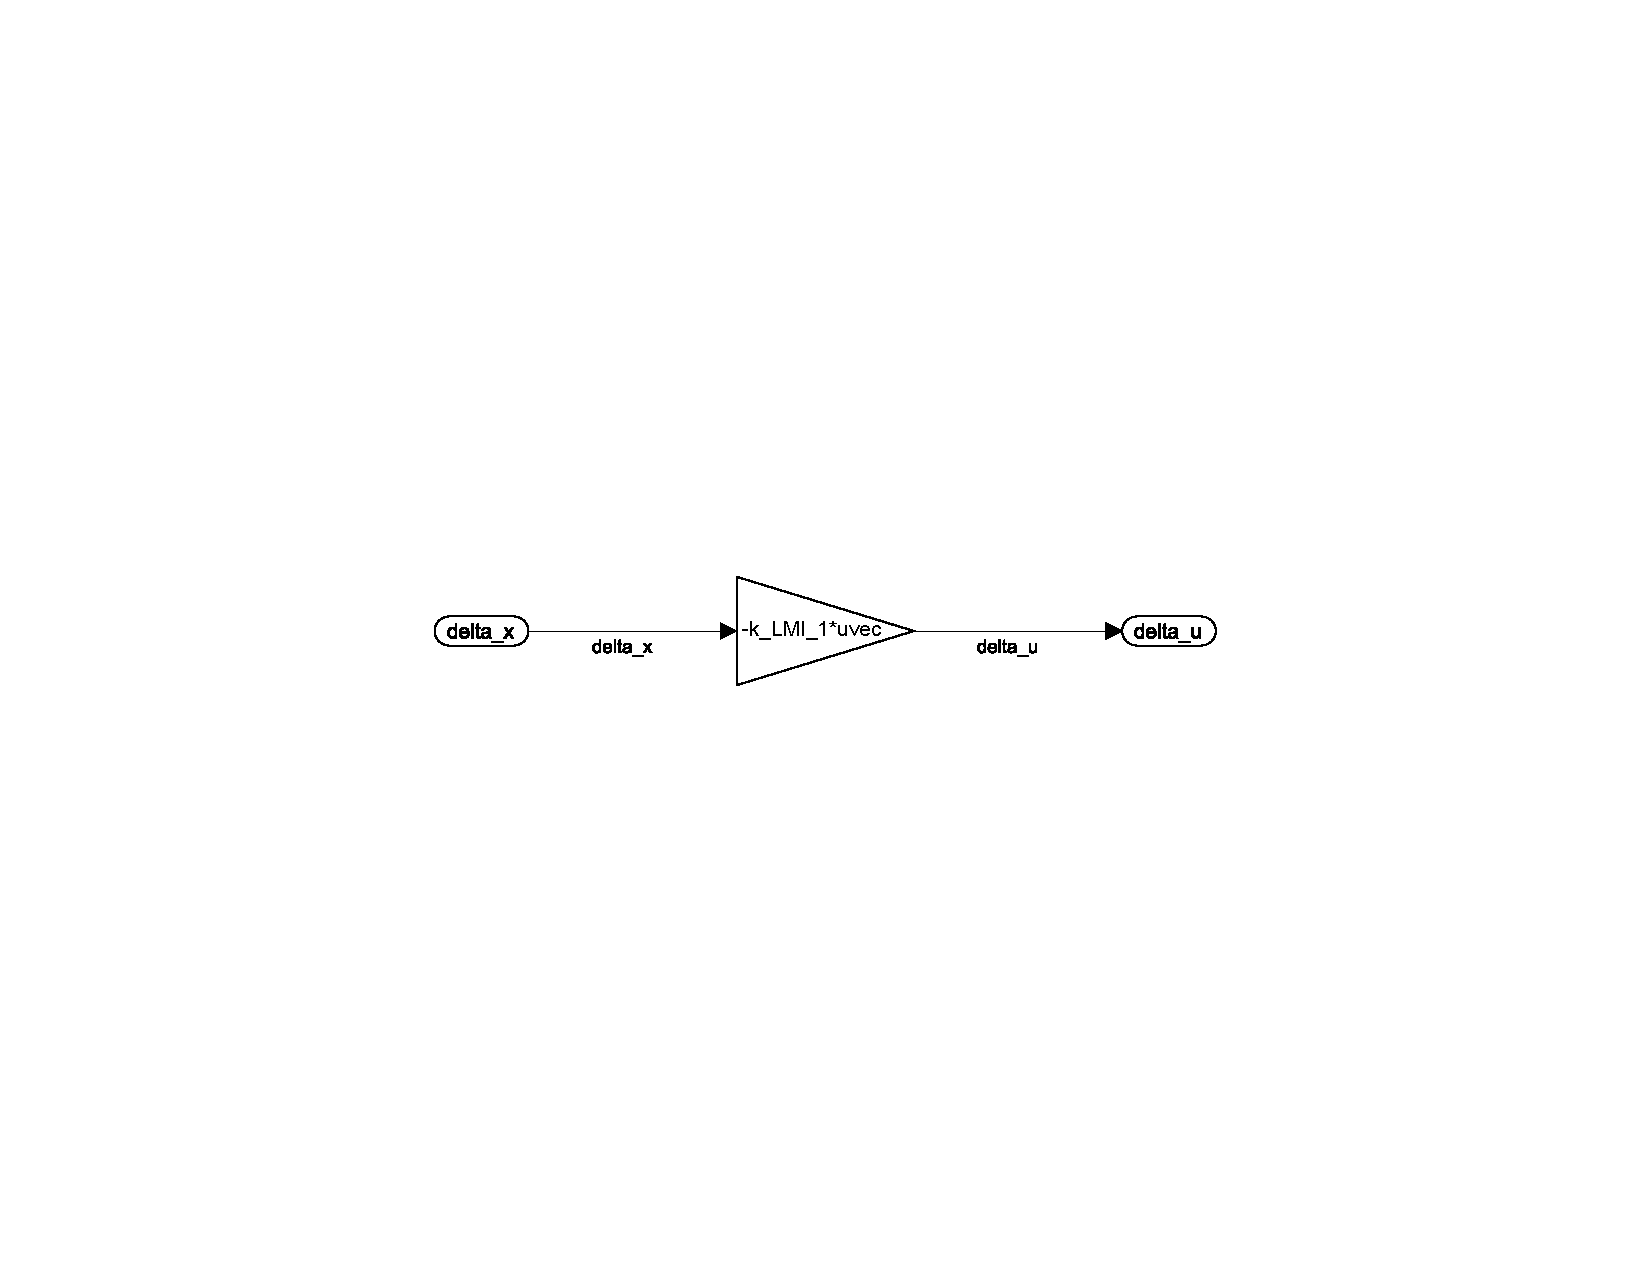
\includegraphics[width=0.65\textwidth]{Bilder/6_reglervalidierung/linear_einfacher_regler_simu.pdf}}
    \caption[Einfacher Zustandsregler Simulink (linear)]{Simulink Regler-Blockschaltbild für den einfachen Zustandsregler (lineares Zustandsraummodell)}
    \label{fig:Bild13}
\end{figure}

Zur Validierung der Funktionsfähigkeit des Reglers wird der Anfangswert der Spannung $v_{\mathrm{PV}}$ um $\SI{10}{V}$ bezogen auf die Ruhelage der PV-Spannung $v_{\mathrm{PV,MPP}}$ abgesenkt. \autoref{fig:Bild14} zeigt, dass der Regler fähig ist, das System wieder in die Ruhelage zu regeln. Dabei wird die Begrenzung der Eingangsgröße $u$, welche zwischen maximal 0 und 1 liegen darf aufgrund der Definition des Duty Cycles, nicht über- oder unterschritten.

\begin{figure}[H]
    \centering
    \fbox{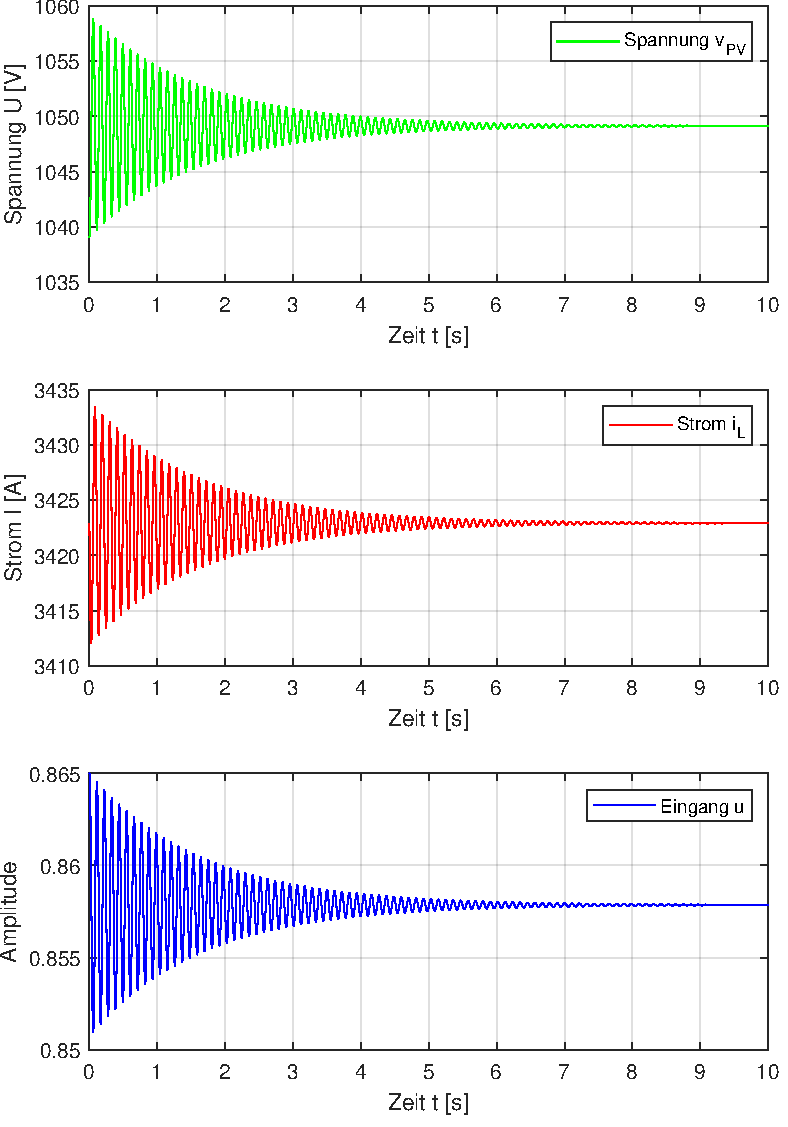
\includegraphics[width=0.85\textwidth]{Bilder/6_reglervalidierung/linear_einfache_rueckfuehrung.pdf}}
    \caption[Validierung Regler mit einfacher Rückführung (linear)]{$v_{\mathrm{PV}}$, $i_{\mathrm{L}}$ und $u$ bei $\alpha = 0.1$ und einem Einganssprung von $v_{\mathrm{PV,MPP}} - \SI{10}{V}$ am einfachen Zustandsregler für das lineare Zustandsraummodell}
    \label{fig:Bild14}
\end{figure}

Es fällt jedoch auf, dass das System stark schwingt und unter anderem dadurch \ca $\SI{8}{s}$ benötigt, um bei einer kleinen initialen Spannungsabweichung wieder zurück in die Ruhelage geregelt zu werden. Das beschriebene Verhalten kann als plausibel erachtet werden, da der Betrag des Imaginärteils der Polstellen um einen Faktor 50 größer ist als der Betrag des Realteils der Polstellen, was aus \autoref{fig:Bild8} hervorgeht. Auf eine Verbesserung dieses Verhaltens über die Anpassung der LMI's wird an dieser Stelle verzichtet. Es konnte nachgewiesen werden, dass der Regler grundsätzlich seine Funktion erfüllt.

\subsubsection{Zustandsregler mit Vorsteuerung} \label{sec:val_lin_vor}

Als nächster Regler wird der Zustandsregler mit Referenzwertvorsteuerung behandelt. Dessen Umsetzung in Simulink kann in \autoref{fig:Bild15} nachvollzogen werden. Ebenfalls wieder simuliert, werden die Zustandsgrößen $v_{\mathrm{PV}}$ und $i_{\mathrm{L}}$ sowie die Eingangsgröße $u$ bei $\alpha = 0.1$ für die Berechnung der k-Faktoren mit LMI's (siehe \autoref{eq:Gleichung23}). Im Unterschied zum vorangegangenen Regler soll es nun auch möglich sein, einen Referenzwert für die PV-Spannung vorzugeben. Dazu wurde in \autoref{eq:Gleichung24} ein Vorfilter $F$ berechnet, über welchen ein Referenzwert $y_{\mathrm{ref}}$ vorgegeben werden kann.

\begin{figure}[H]
    \centering
    \fbox{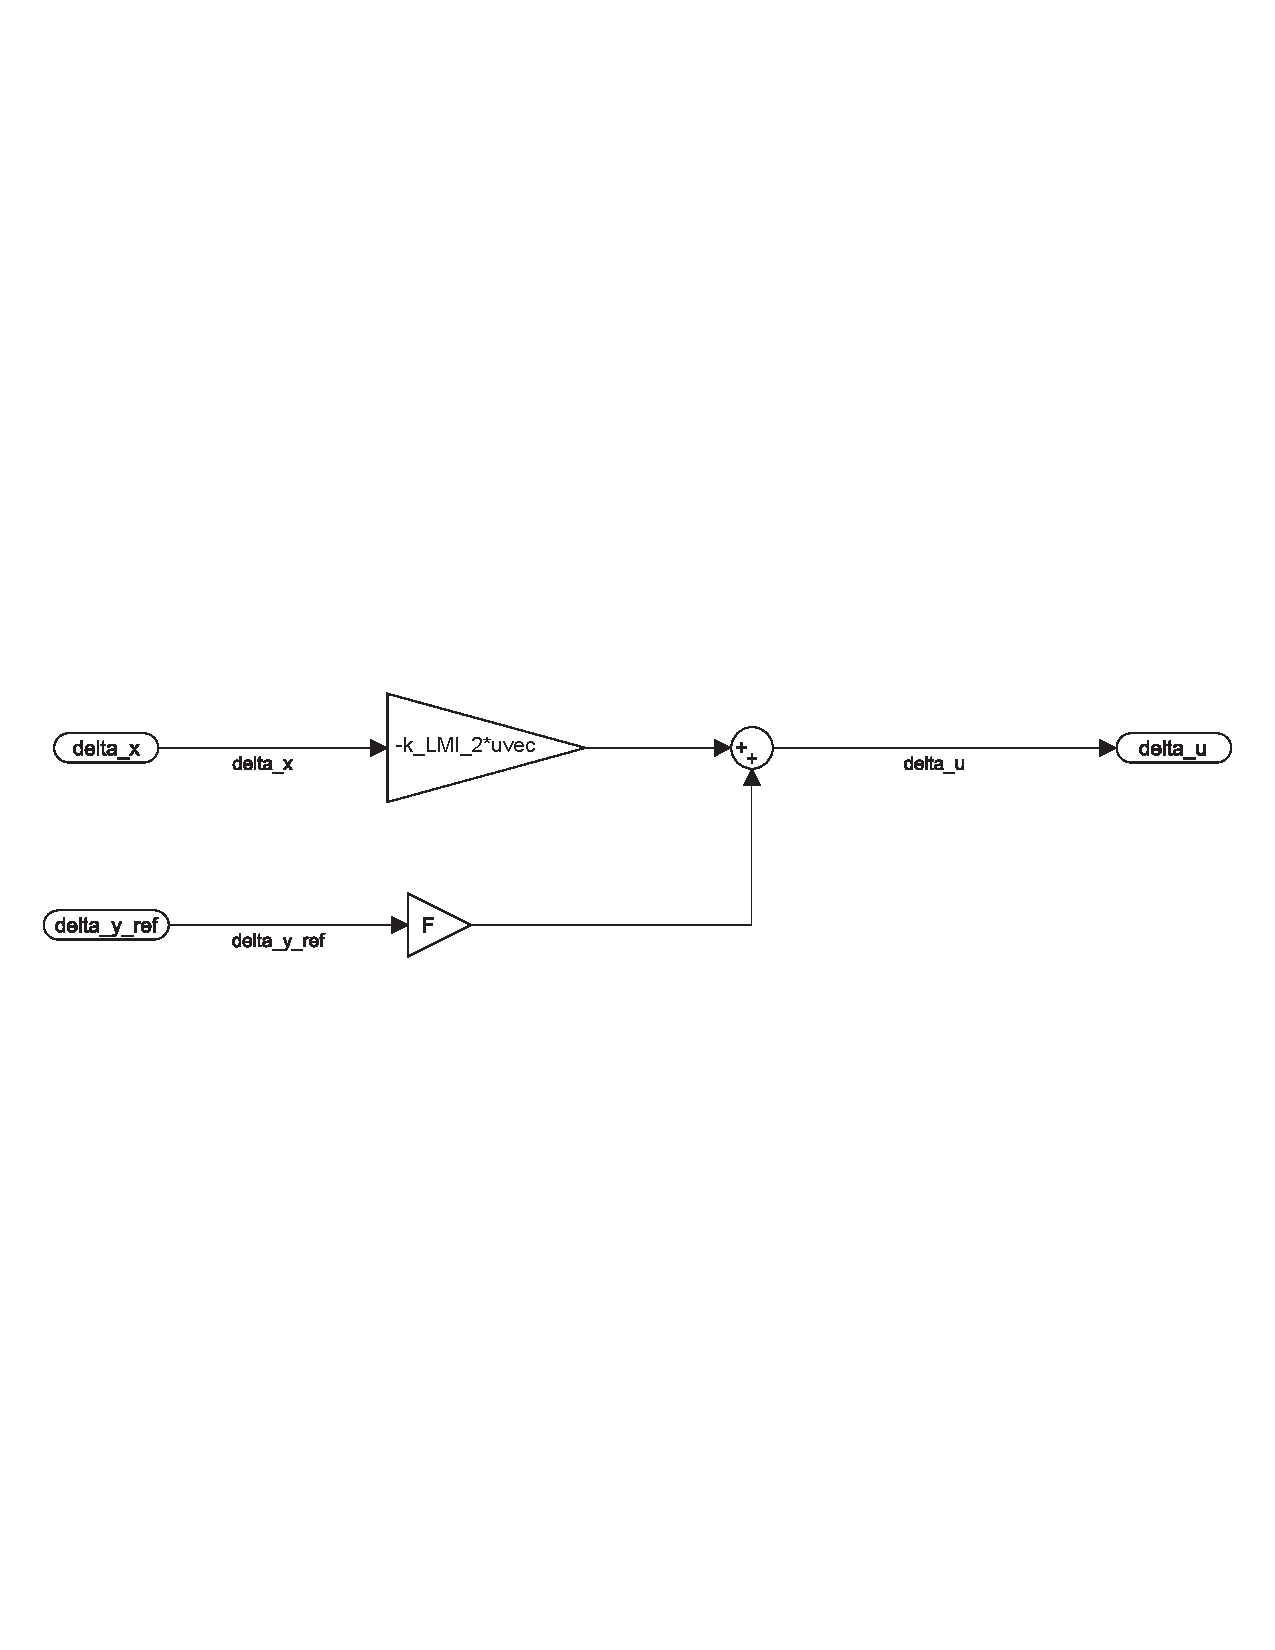
\includegraphics[width=1.0\textwidth]{Bilder/6_reglervalidierung/linear_vorsteuerung_simu.pdf}}
    \caption[Zustandsregler mit Vorsteuerung Simulink (linear)]{Simulink Regler-Blockschaltbild für den Zustandsregler mit Vorsteuerung (lineares Zustandsraummodell)}
    \label{fig:Bild15}
\end{figure}

Zur Validierung der Funktionsfähigkeit des Reglers wird ein Referenzwert von $\SI{+10}{V}$ bezogen für die PV-Spannung $v_{\mathrm{PV,MPP}}$ vorgegeben. \autoref{fig:Bild16} zeigt, dass der Regler fähig ist das System zum angegeben Referenzwert auszuregeln. Dabei wird die Begrenzung der Eingangsgröße von $u \in \mathbb{R} \: | \: 0 \leq u \leq 1$ nicht über- oder unterschritten. \\
Auch hier fällt auf, dass das System stark schwingt und erneut rund $\SI{8}{s}$ benötigt, um den gewünschten Referenzwert zu erreichen. Die Begründung findet sich ebenfalls in der Lage der Polstellen, bei welchen der Betrag des Imaginärteils 50-fach größer ist als der Betrag des Realteils (siehe \autoref{fig:Bild10}).

\begin{figure}[H]
    \centering
    \fbox{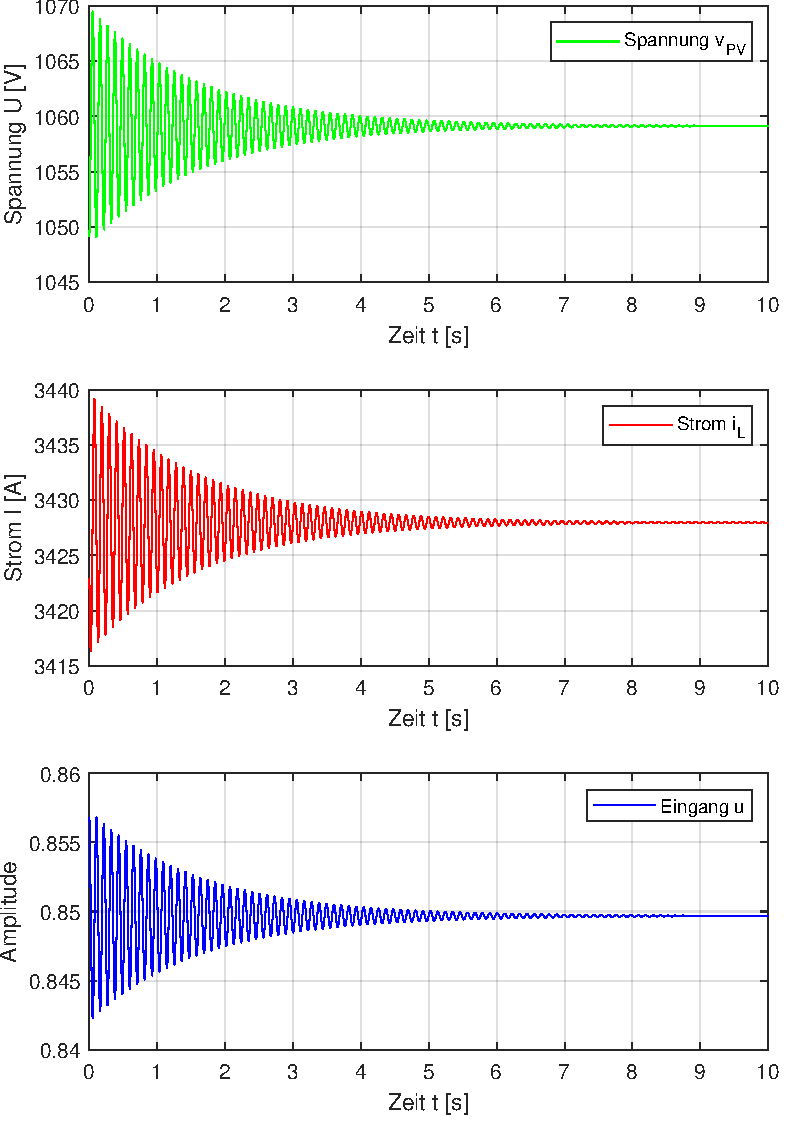
\includegraphics[width=0.85\textwidth]{Bilder/6_reglervalidierung/linear_referenzwertvorsteuerung.pdf}}
    \caption[Validierung Regler mit Vorsteuerung (linear)]{$v_{\mathrm{PV}}$, $i_{\mathrm{L}}$ und $u$ bei $\alpha = 0.1$ und einem Referenzwert von $y_{ref} = v_{\mathrm{PV,MPP}} + \SI{10}{V}$ am Zustandsregler mit Referenzwertvorsteuerung für das lineare Zustandsraummodell}
    \label{fig:Bild16}
\end{figure}

\subsubsection{Zustandsregler mit I-Regelung}

Der dritte umgesetzte Zustandsregler ist der I-Regler. Die Implementation für Simulink ist in \autoref{fig:Bild17} dargestellt. Auch hier werden die Zustandsgrößen $v_{\mathrm{PV}}$ und $i_{\mathrm{L}}$ sowie die Eingangsgröße $u$ bei $\alpha = 0.1$ für die Berechnung der k-Faktoren mit LMI's (siehe \autoref{eq:Gleichung29}) simuliert. Abweichend zu den vorherigen Reglern wird zunächst das erweiterte Zustandsraummodell aufgestellt (\autoref{eq:Gleichung28}), über welches die Tilde-Matrizen für die A- und B-Matrix erhalten werden können. Mit Hilfe dieser werden nun drei statt zwei k-Faktoren über LMI's berechnet. Wie auch schon bei der Referenzwertvorsteuerung ist es möglich einen Referenzwert $y_{\mathrm{ref}}$ vorzugeben. Der wesentliche Unterschied zur Vorsteuerung liegt im Aufintegrieren des Regelfehlers, wodurch eine generelle Optimierung des Regelverhaltens zu erwarten ist.

\begin{figure}[H]
    \centering
    \fbox{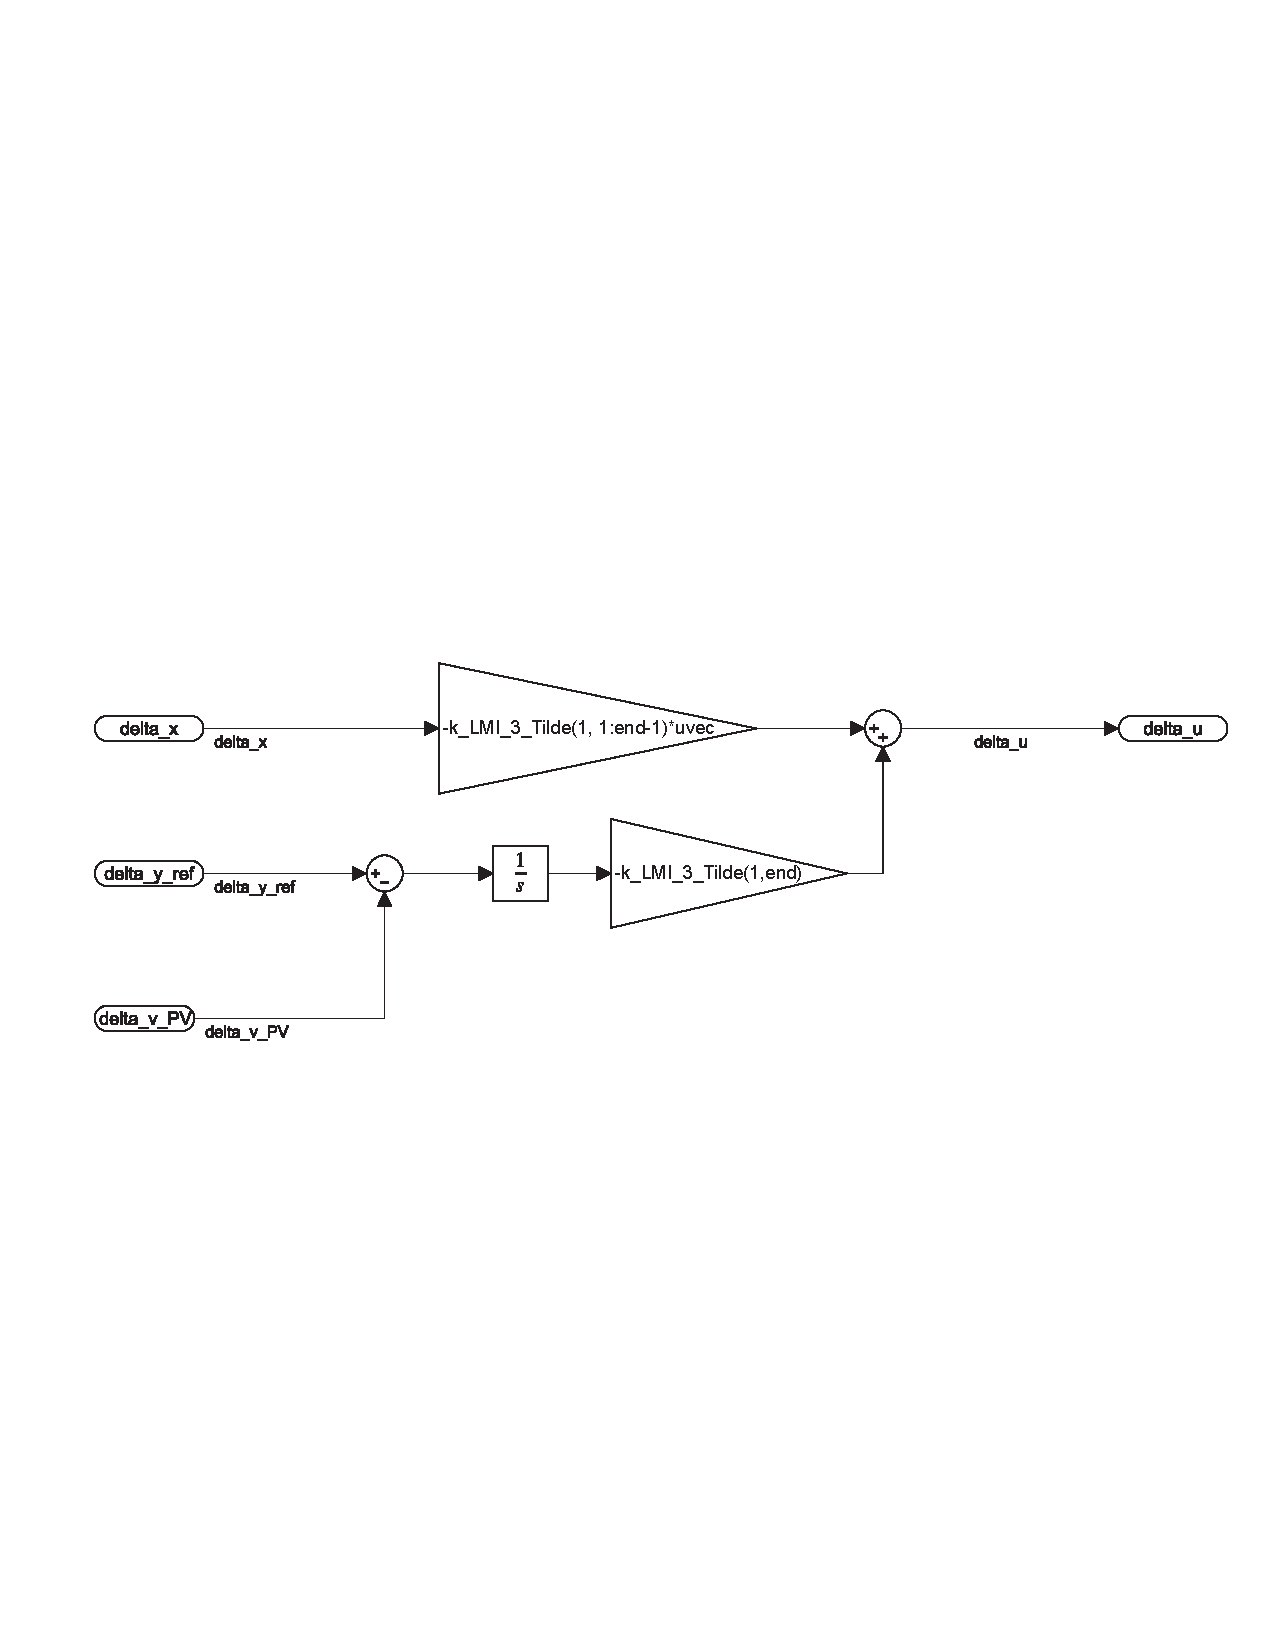
\includegraphics[width=1.0\textwidth]{Bilder/6_reglervalidierung/linear_i_regler_simu.pdf}}
    \caption[Zustandsregler mit I-Regelung Simulink (linear)]{Simulink Regler-Blockschaltbild für den Zustandsregler mit I-Regelung (lineares Zustandsraummodell)}
    \label{fig:Bild17}
\end{figure}

Zur Validierung der Funktionsfähigkeit des Reglers wird erneut ein Referenzwert von $\SI{+10}{V}$ bezogen für die PV-Spannung $v_{\mathrm{PV,MPP}}$ vorgegeben. \autoref{fig:Bild18} zeigt, dass der Regler fähig ist das System zum angegeben Referenzwert auszuregeln. Dabei wird die Begrenzung der Eingangsgröße von $u \in \mathbb{R} \: | \: 0 \leq u \leq 1$ nicht über- oder unterschritten. \\
Es kann positiv vermerkt werden, dass das System im Vergleich zu den vorangegangenen Reglern nur noch minimal schwingt. Grund dafür ist vermutlich die dritte Polstelle (siehe \autoref{fig:Bild12}), die im Vergleich zu den ersten beiden keinen Imaginärteil aufweist und damit das System weniger schwingungsfähig macht. Begründet durch die höhere Komplexität des Reglers dauert der Vorgang des Ausregelns zu dem gewünschten Referenzwert jedoch \ca $\SI{2}{s}$ länger als beim Zustandsregler mit Referenzwertvorsteuerung.

\begin{figure}[H]
    \centering
    \fbox{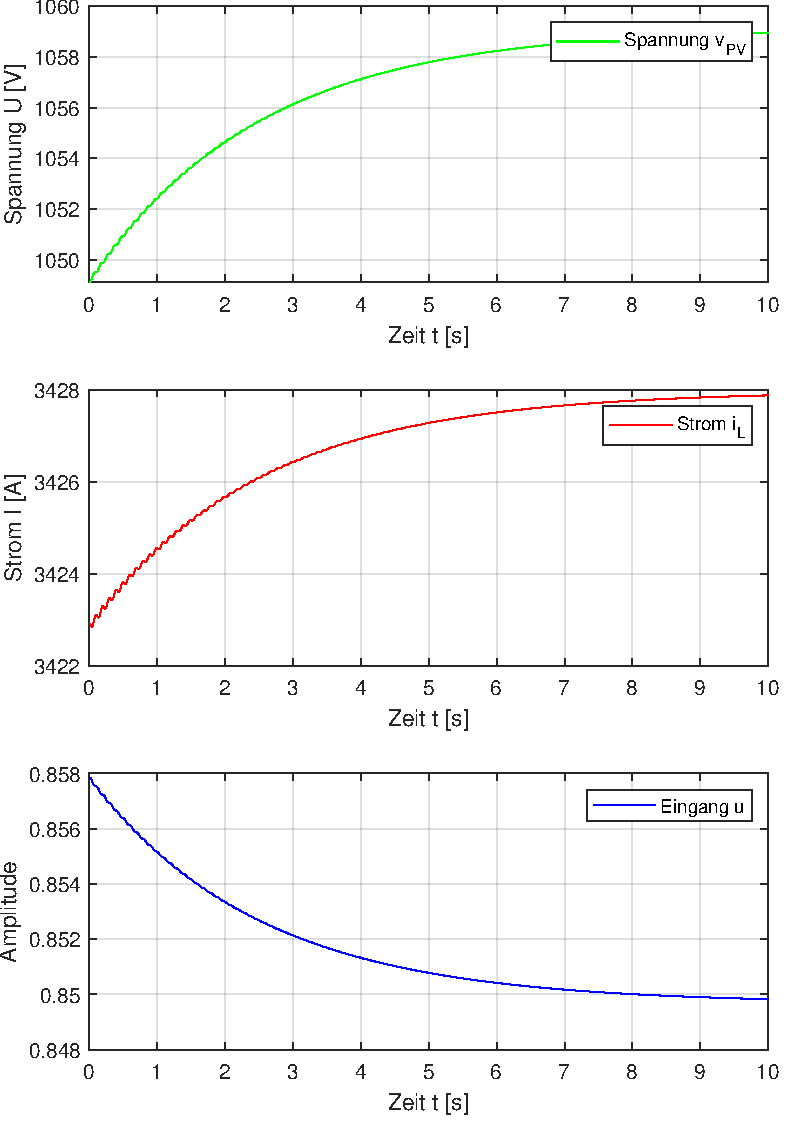
\includegraphics[width=0.85\textwidth]{Bilder/6_reglervalidierung/linear_i_regelung.pdf}}
    \caption[Validierung Regler mit I-Regelung (linear)]{$v_{\mathrm{PV}}$, $i_{\mathrm{L}}$ und $u$ bei $\alpha = 0.1$ und einem Referenzwert von $y_{ref} = v_{\mathrm{PV,MPP}} + \SI{10}{V}$ am Zustandsregler mit I-Regelung für das lineare Zustandsraummodell}
    \label{fig:Bild18}
\end{figure}

\subsubsection{Vergleich des Regelverhaltens}

Abschließend wird ein Vergleich der drei Regelkonzepte für das lineare Zustandsraummodell vorgenommen. Dabei werden die Regler bezüglich der Performance gegenübergestellt. Um einen konkreten Vergleich vornehmen zu können, wurden die Kurvenverläufe, die bereits auf den vorhergehenden Seiten gezeigt worden sind, für die Größen $v_{\mathrm{PV}}$, $i_{\mathrm{L}}$ und $u$ übereinander gelegt. \autoref{fig:Bild19} zeigt den Vergleich der drei Zustandsregler. \\
\newline
Es ist zunächst offensichtlich, dass ein wesentlicher Unterschied zwischen dem Regler mit einfacher Zustandsrückführung und den beiden Reglern mit der Fähigkeit einen Referenzwert entgegenzunehmen besteht. Durch die Referenzwertvorgabe für die Spannung $v_{\mathrm{PV}}$ bei einem Referenzwert von $\SI{+10}{V}$ bezogen für die PV-Spannung $v_{\mathrm{PV,MPP}}$ ist der Endwert für den Zustandsregler mit Vorsteuerung und für den Zustandsregler mit I-Regelung um $\SI{10}{V}$ größer. Dies ist im Spannungsdiagramm in \autoref{fig:Bild19} ersichtlich.\\
Durch die angepasste Spannung ändert sich auch der Strom $i_{\mathrm{L}}$ und der Eingang $u$ anti-proportional zu der Differenz des Referenzwertes bezogen auf die Ruhelage.\\
\newline
Weiterhin ist zu erkennen, dass die Geschwindigkeit der drei Regler voneinander abweicht, obwohl für die Berechnung der k-Faktoren der Zustandsregler das selbe $\alpha$ ($\alpha = 0.1$) verwendet wurde. In der \autoref{fig:Bild19} ist zu erkennen, dass die Hüllkurve des einfachen Zustandsreglers und die des Reglers mit Vorsteuerung annähernd identisch sind. Vergleicht man diese jedoch mit dem Kurvenverlauf des I-Reglers kann ermittelt werden, dass dieser, was das Ausregeln der Zustandsgröße $v_{\mathrm{PV}}$ angeht, etwas langsamer scheint. Dieses Phänomen ergibt sich vermutlich aus dem weiteren k-Faktor bei der I-Regelung und der damit einhergehenden erhöhten Komplexität, nicht zuletzt auch durch die ebenfalls dazugekommene Integration.\\
\newline
Bei der Betrachtung des Zustandsreglers mit I-Regelung im Vergleich zu den anderen beiden Regelkonzepten fällt auf, dass die Schwingungen stark reduziert sind. Dabei handelt es sich um einen wünschenswerten Effekt, der maßgeblich durch die Polstellenlage beeinflusst wird. Der I-Regler besitzt eine weitere Polstelle, welche rein reell ist und damit dämpfend gegenüber den Polstellen mit großem Imaginärteil wirkt.

\begin{figure}[H]
    \centering
    \fbox{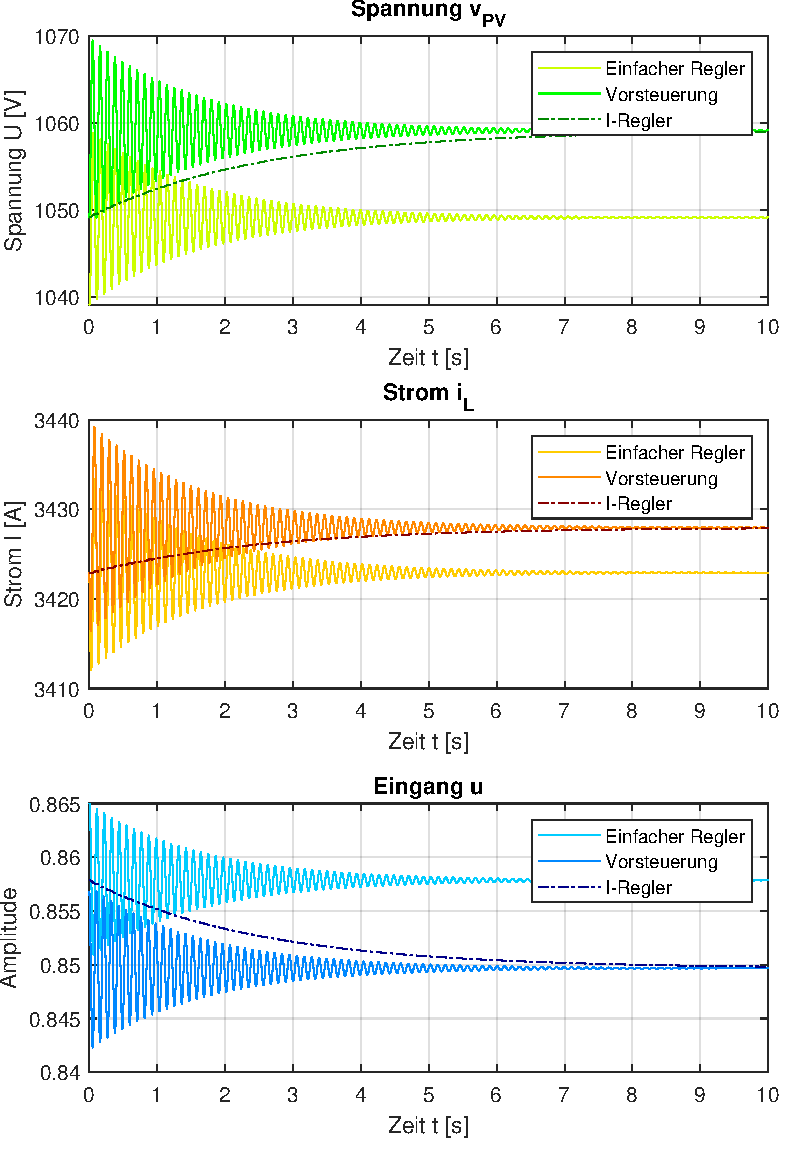
\includegraphics[width=0.8\textwidth]{Bilder/6_reglervalidierung/linear_reglervergleich.pdf}}
    \caption[Reglervergleich für das lineare Zustandsraummodell]{$v_{\mathrm{PV}}$, $i_{\mathrm{L}}$ und $u$ für Regler mit einfacher Zustandsrückführung, Regler mit Referenzwertvorsteuerung und Regler mit I-Regelung bei einem Einganssprung von $v_{\mathrm{PV,MPP}} - \SI{10}{V}$ \bzw einem Referenzwert von $y_{ref} = v_{\mathrm{PV,MPP}} + \SI{10}{V}$ am linearen Zustandsraummodell}
    \label{fig:Bild19}
\end{figure}

\subsection{Validierung des nichtlinearen Modells} \label{sec:Vergleich_nichtlinear}

Der zweite Unterabschnitt behandelt die Validierung der Regler am nichtlinearen Zustandsraummodell. Die nichtlineare Strecke wurde bereits in Simulink umgesetzt und ist in \autoref{fig:Bild3} dargestellt. Bei der Umsetzung der Regler für das nichtlinearen Modell ist wichtig zu beachten, dass ausschließlich der Regler mit Delta-Größen arbeitet, die Regelstrecke im Vergleich zum linearen Modell jedoch nicht. Für die Ausgabe der Zustandsvektoren $v_{\mathrm{PV}}$ und $i_{\mathrm{L}}$ in Diagrammform können direkt die Ausgänge der Regelstrecke visualisiert werden. Die Eingangsgröße $u$ muss weiterhin mit dem Duty Cycle $d$ verrechnet werden. Da die Zustandsvektoren auf den Regler zurückgeführt sind, muss am Eingang des Reglers die jeweilige Ruhelage subtrahiert werden. Dieser Zusammenhang ist beispielsweise in \autoref{fig:Bild20} auf der linken Seite zu erkennen. 

\subsubsection{Zustandsregler mit einfacher Zustandsrückführung}

Erneut wird mit dem Zustandsregler mit einfacher Rückführung begonnen. Das Simulink-Blockschaltbild ist in \autoref{fig:Bild20} gezeigt. Simuliert werden die Zustandsgrößen $v_{\mathrm{PV}}$ und $i_{\mathrm{L}}$ sowie die Eingangsgröße $u$ bei $\alpha = 0.1$ für die Berechnung der k-Faktoren mit LMI's (siehe \autoref{eq:Gleichung21}).

\begin{figure}[H]
    \centering
    \fbox{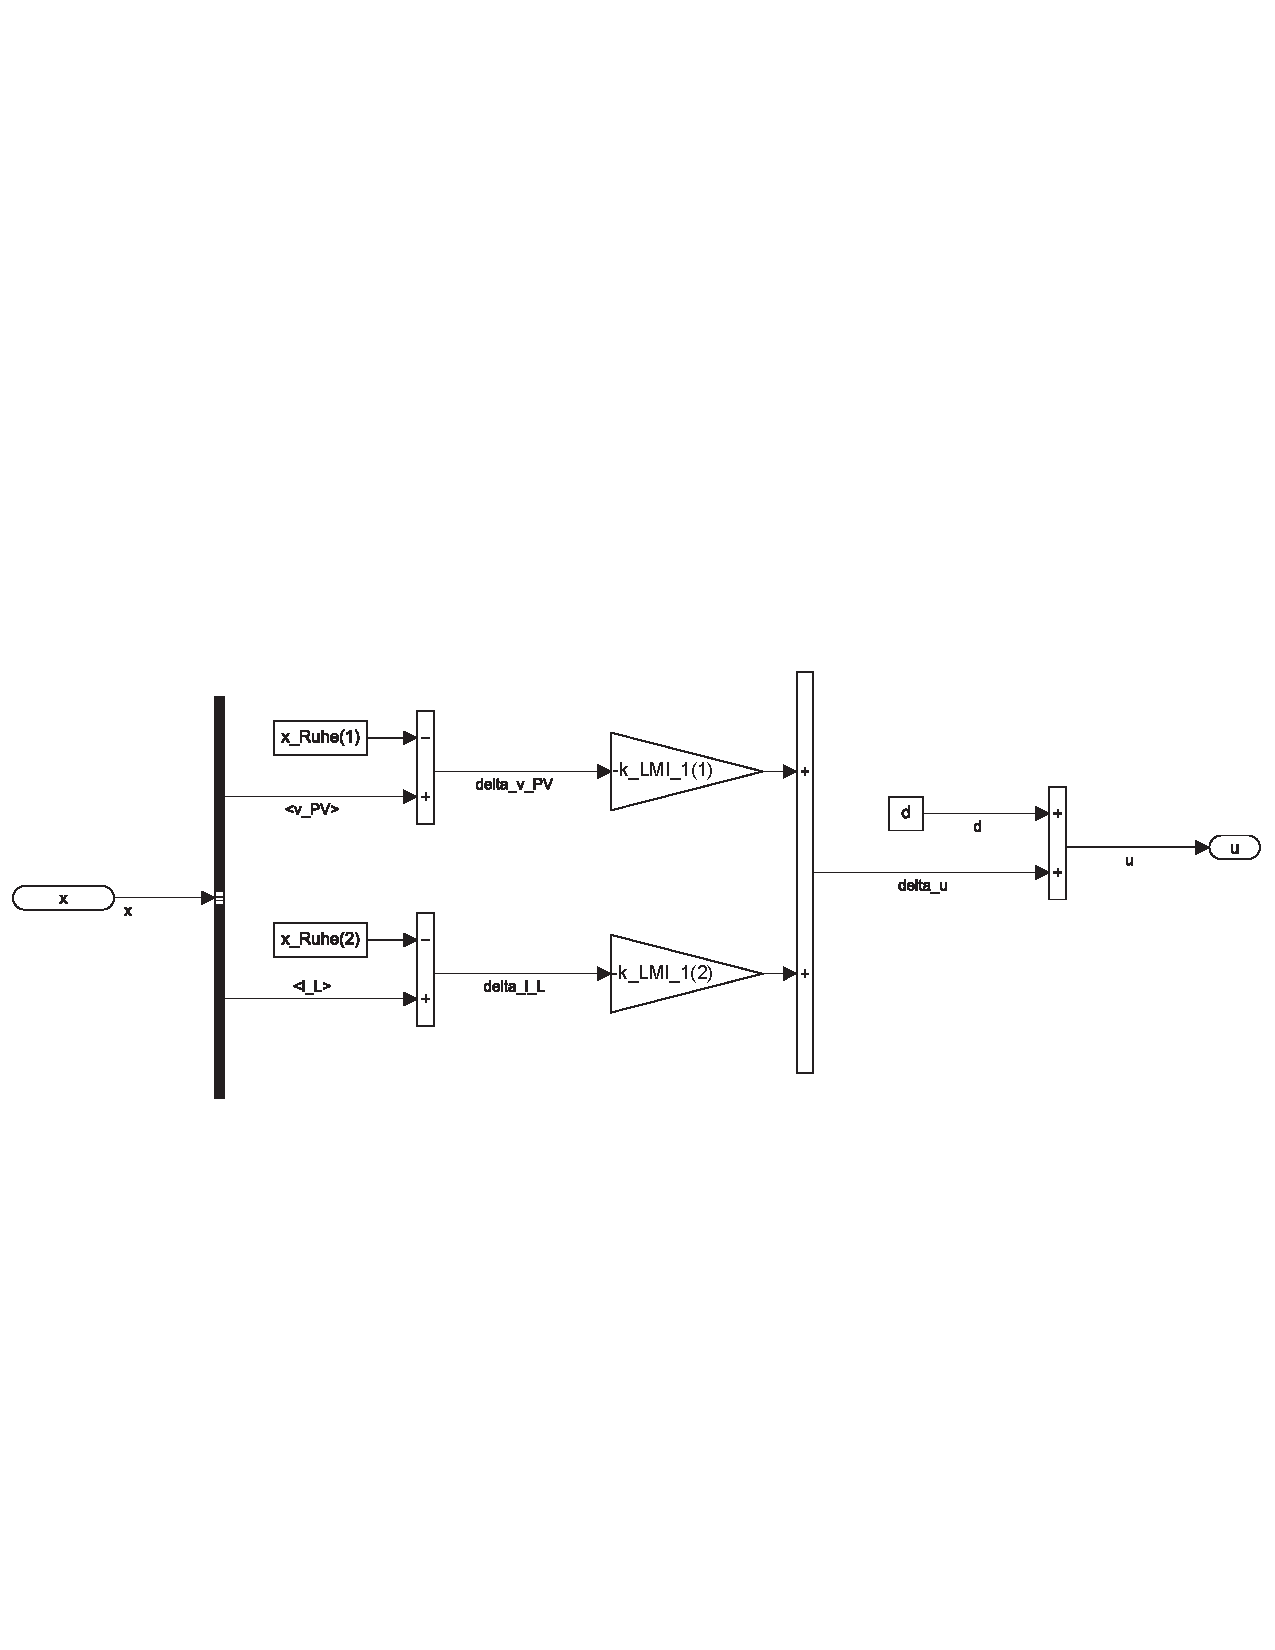
\includegraphics[width=1.0\textwidth]{Bilder/6_reglervalidierung/nichtlinear_einfacher_regler_simu.pdf}}
    \caption[Einfacher Zustandsregler Simulink (nicht-linear)]{Simulink Regler-Blockschaltbild für den einfachen Zustandsregler (nichtlineares Zustandsraummodell)}
    \label{fig:Bild20}
\end{figure}

Zur Validierung der Funktionsfähigkeit des Reglers wird der Anfangswert der Spannung $v_{\mathrm{PV}}$ um $\SI{10}{V}$ bezogen auf die Ruhelage der PV-Spannung $v_{\mathrm{PV,MPP}}$ abgesenkt. \autoref{fig:Bild21} zeigt nahezu identische Ergebnisse im Vergleich zum linearen Zustandsraummodell. Aufgrund dieser Erkenntnis wird auf weitere Analysen verzichtet.

\begin{figure}[H]
    \centering
    \fbox{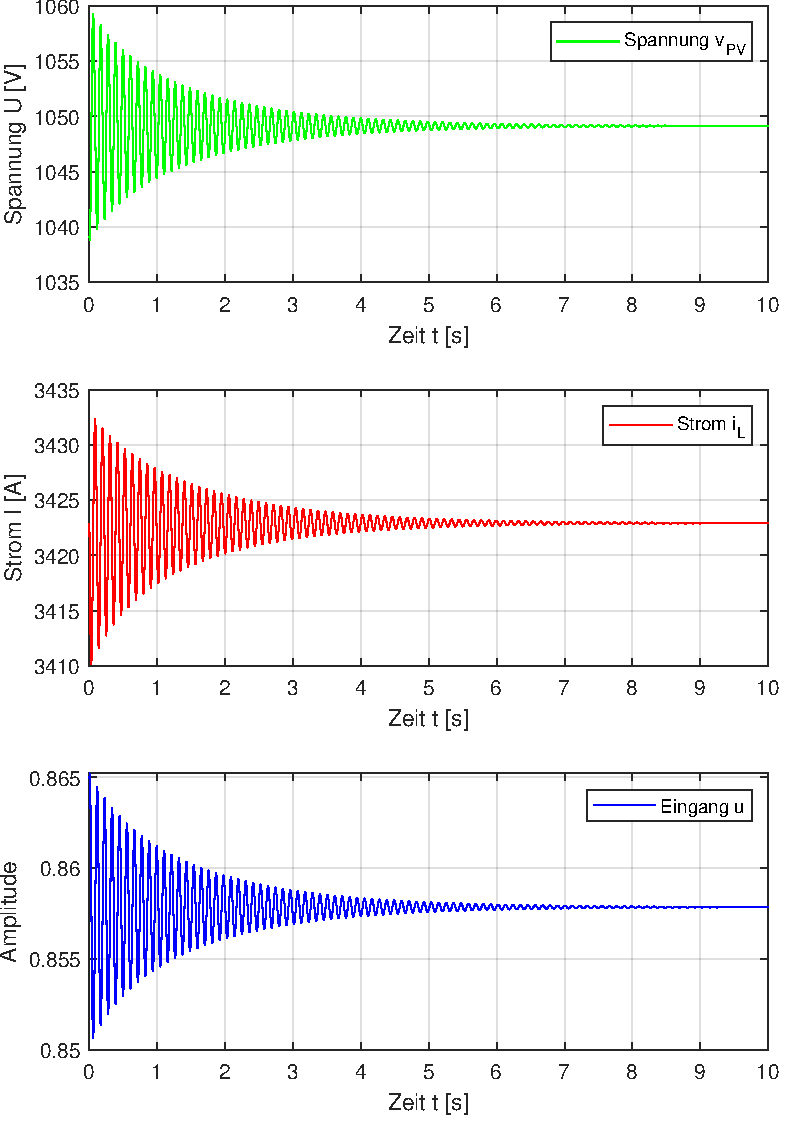
\includegraphics[width=0.85\textwidth]{Bilder/6_reglervalidierung/nichtlinear_einfache_rueckfuehrung.pdf}}
    \caption[Validierung Regler mit einfacher Rückführung (nichtlinear)]{$v_{\mathrm{PV}}$, $i_{\mathrm{L}}$ und $u$ bei $\alpha = 0.1$ und einem Einganssprung von $v_{\mathrm{PV,MPP}} - \SI{10}{V}$ am einfachen Zustandsregler für das nichtlineare Zustandsraummodell}
    \label{fig:Bild21}
\end{figure}

\subsubsection{Zustandsregler mit Vorsteuerung} \label{sec:val_nlin_vor}

Nachfolgend wird der Zustandsregler mit Referenzwertvorsteuerung auf das nichtlineare Zustandsraummodell angewendet. Die Umsetzung des Reglers in Simulink kann in \autoref{fig:Bild22} nachvollzogen werden. Ebenfalls wieder simuliert, werden die Zustandsgrößen $v_{\mathrm{PV}}$ und $i_{\mathrm{L}}$ sowie die Eingangsgröße $u$ bei $\alpha = 0.1$ für die Berechnung der k-Faktoren mit LMI's (siehe \autoref{eq:Gleichung23}). Im Unterschied zum vorangegangenen Regler Soll es nun auch möglich sein, einen Referenzwert für die PV-Spannung vorzugeben. Dazu wurde in \autoref{eq:Gleichung24} ein Vorfilter $F$ berechnet, über welchen ein Referenzwert $y_{\mathrm{ref}}$ vorgegeben werden kann.

\begin{figure}[H]
    \centering
    \fbox{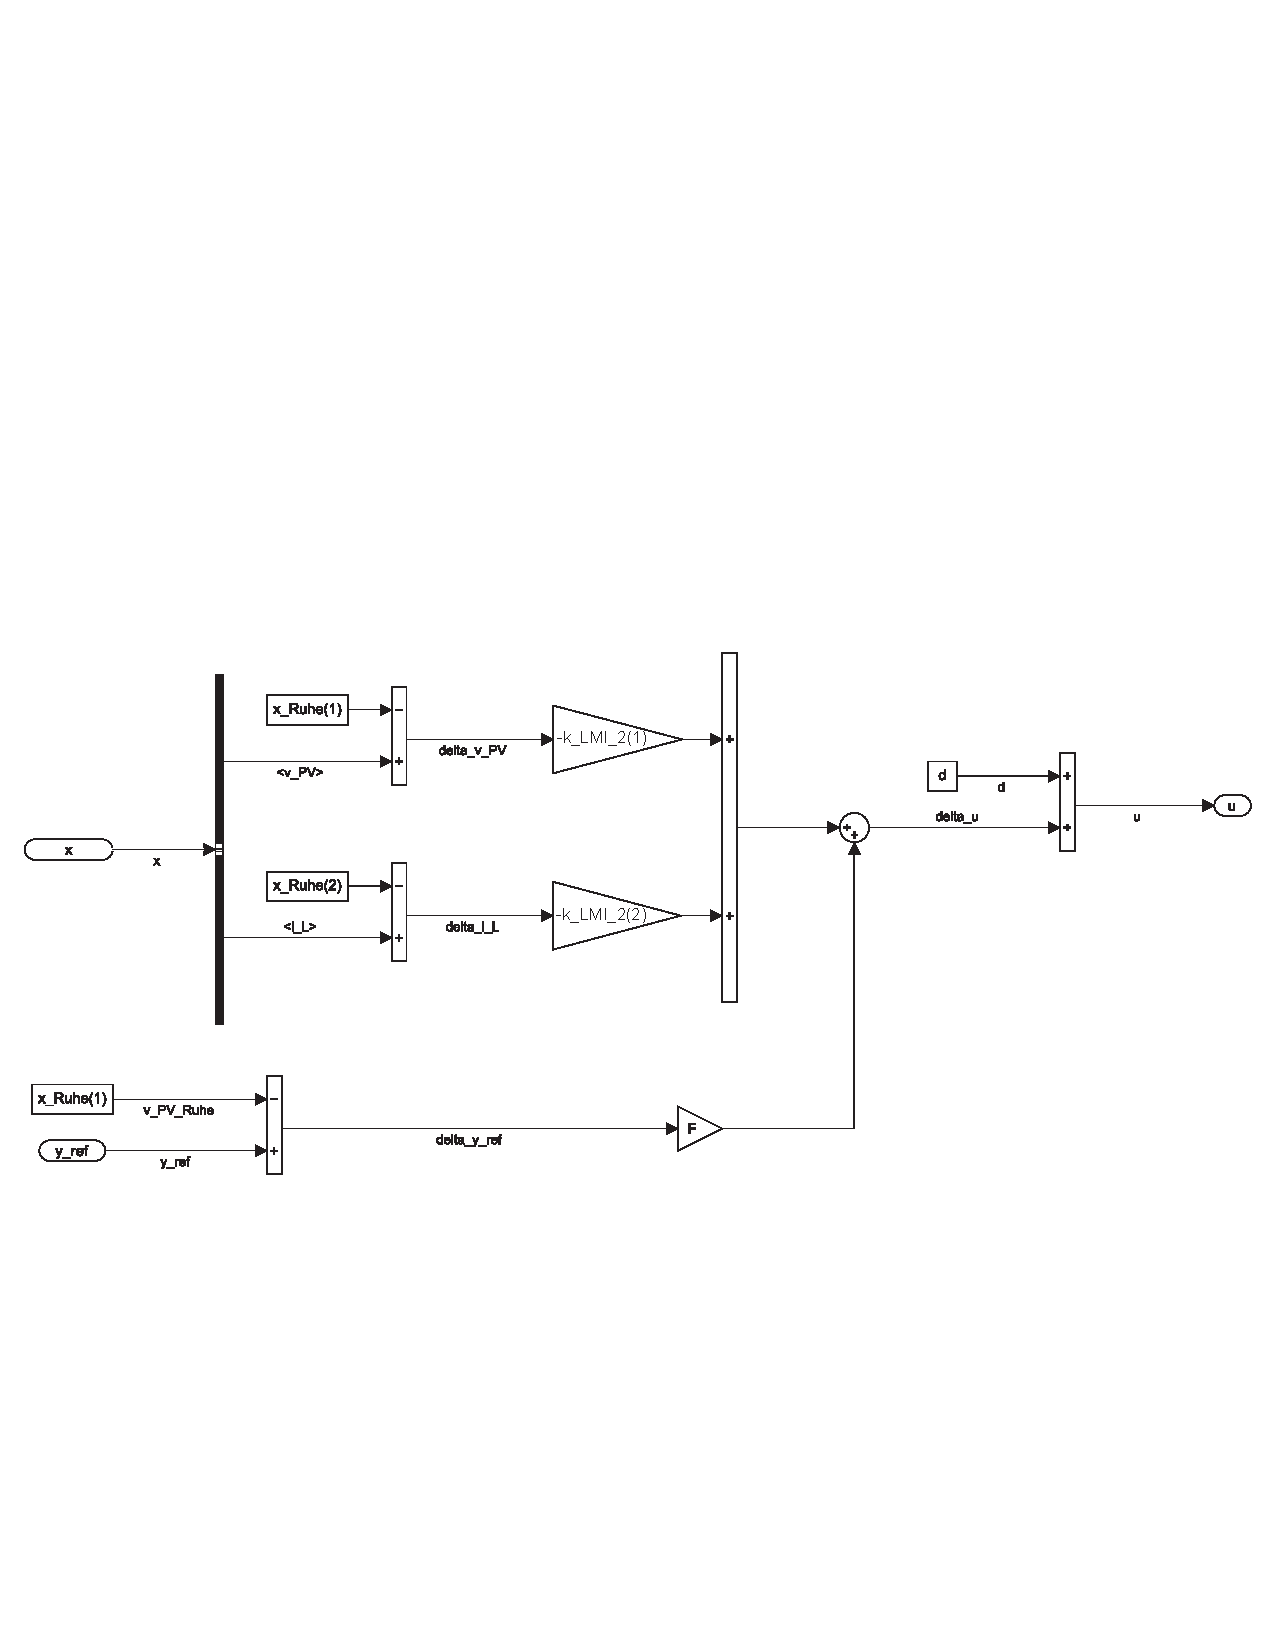
\includegraphics[width=1.0\textwidth]{Bilder/6_reglervalidierung/nichtlinear_vorsteuerung_simu.pdf}}
    \caption[Zustandsregler mit Vorsteuerung Simulink (nichtlinear)]{Simulink Regler-Blockschaltbild für den Zustandsregler mit Vorsteuerung (nichtlineares Zustandsraummodell)}
    \label{fig:Bild22}
\end{figure}

Bei der Betrachtung der Ergebnisse aus \autoref{fig:Bild23} fällt auf, dass sowohl die Spannung $v_{\mathrm{PV}}$, der Strom $i_{\mathrm{L}}$ und der Eingang $u$ von den Simulationsergebnissen aus \autoref{sec:val_lin_vor} signifikant abweichen. Das System schwingt nur kurz und ist in unter $\SI{500}{ms}$ zum Referenzwert ausgeregelt. Es scheint, als wäre die Performance des Reglers stark gesteigert. Es handelt sich jedoch vermutlich um die Auswirkungen des Regelfehlers bei der Referenzwertvorsteuerung, welche sich offensichtlich positiv auf das Regelverhalten auswirken.

\begin{figure}[H]
    \centering
    \fbox{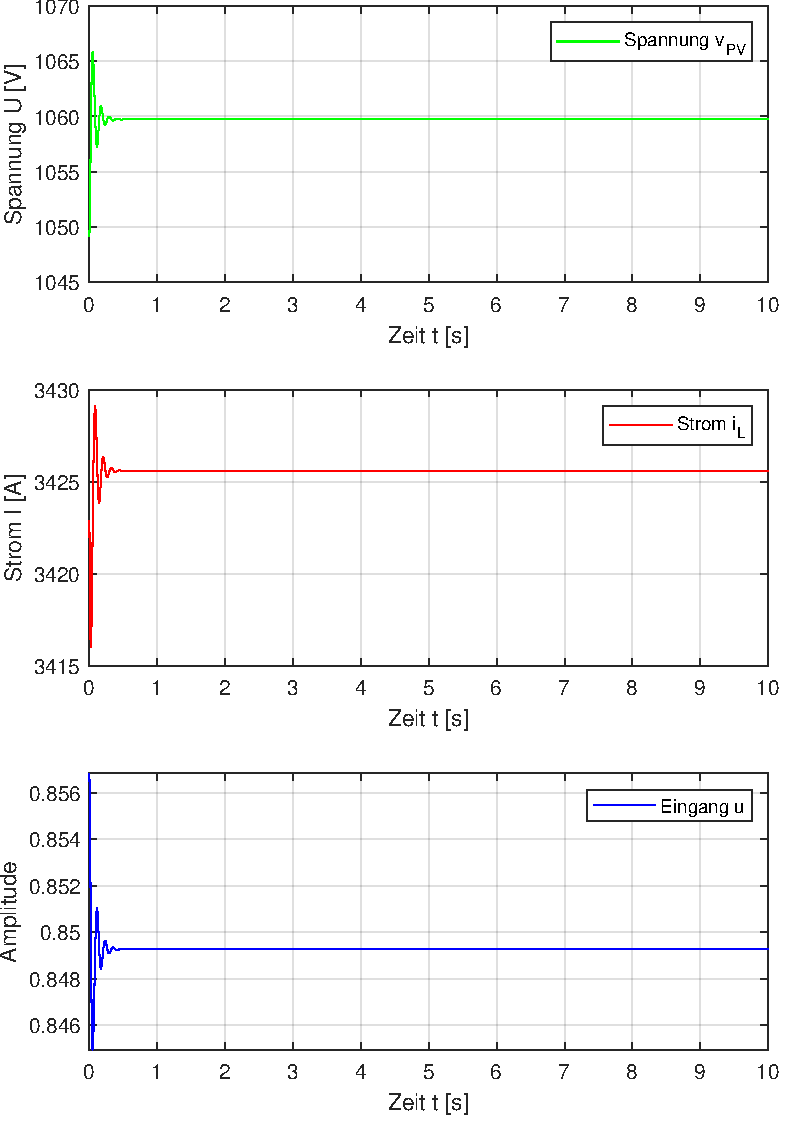
\includegraphics[width=0.85\textwidth]{Bilder/6_reglervalidierung/nichtlinear_referenzwertvorsteuerung.pdf}}
    \caption[Validierung Regler mit Vorsteuerung (nichtlinear)]{$v_{\mathrm{PV}}$, $i_{\mathrm{L}}$ und $u$ bei $\alpha = 0.1$ und einem Referenzwert von $y_{ref} = v_{\mathrm{PV,MPP}} + \SI{10}{V}$ am Zustandsregler mit Referenzwertvorsteuerung für das nichtlineare Zustandsraummodell}
    \label{fig:Bild23}
\end{figure}

\subsubsection{Zustandsregler mit I-Regelung}

Der zuletzt umgesetzte Zustandsregler ist der I-Regler für das nichtlineare Zustandsraummodell. Die Implementation für Simulink ist in \autoref{fig:Bild24} dargestellt. Auch hier werden die Zustandsgrößen $v_{\mathrm{PV}}$ und $i_{\mathrm{L}}$ sowie die Eingangsgröße $u$ bei $\alpha = 0.1$ für die Berechnung der k-Faktoren mit LMI's (siehe \autoref{eq:Gleichung29}) simuliert. Abweichend zu den vorherigen Reglern wird zunächst das erweiterte Zustandsraummodell aufgestellt (\autoref{eq:Gleichung28}), über welches die Tilde-Matrizen für die A- und B-Matrix erhalten werden können. Mit Hilfe dieser werden nun drei statt zwei k-Faktoren über LMI's berechnet. Wie auch schon bei der Referenzwertvorsteuerung ist es möglich einen Referenzwert $y_{\mathrm{ref}}$ vorzugeben. Der wesentliche Unterschied zur Vorsteuerung liegt im Aufintegrieren des Regelfehlers, wodurch eine generelle Optimierung des Regelverhaltens zu erwarten ist.

\begin{figure}[H]
    \centering
    \fbox{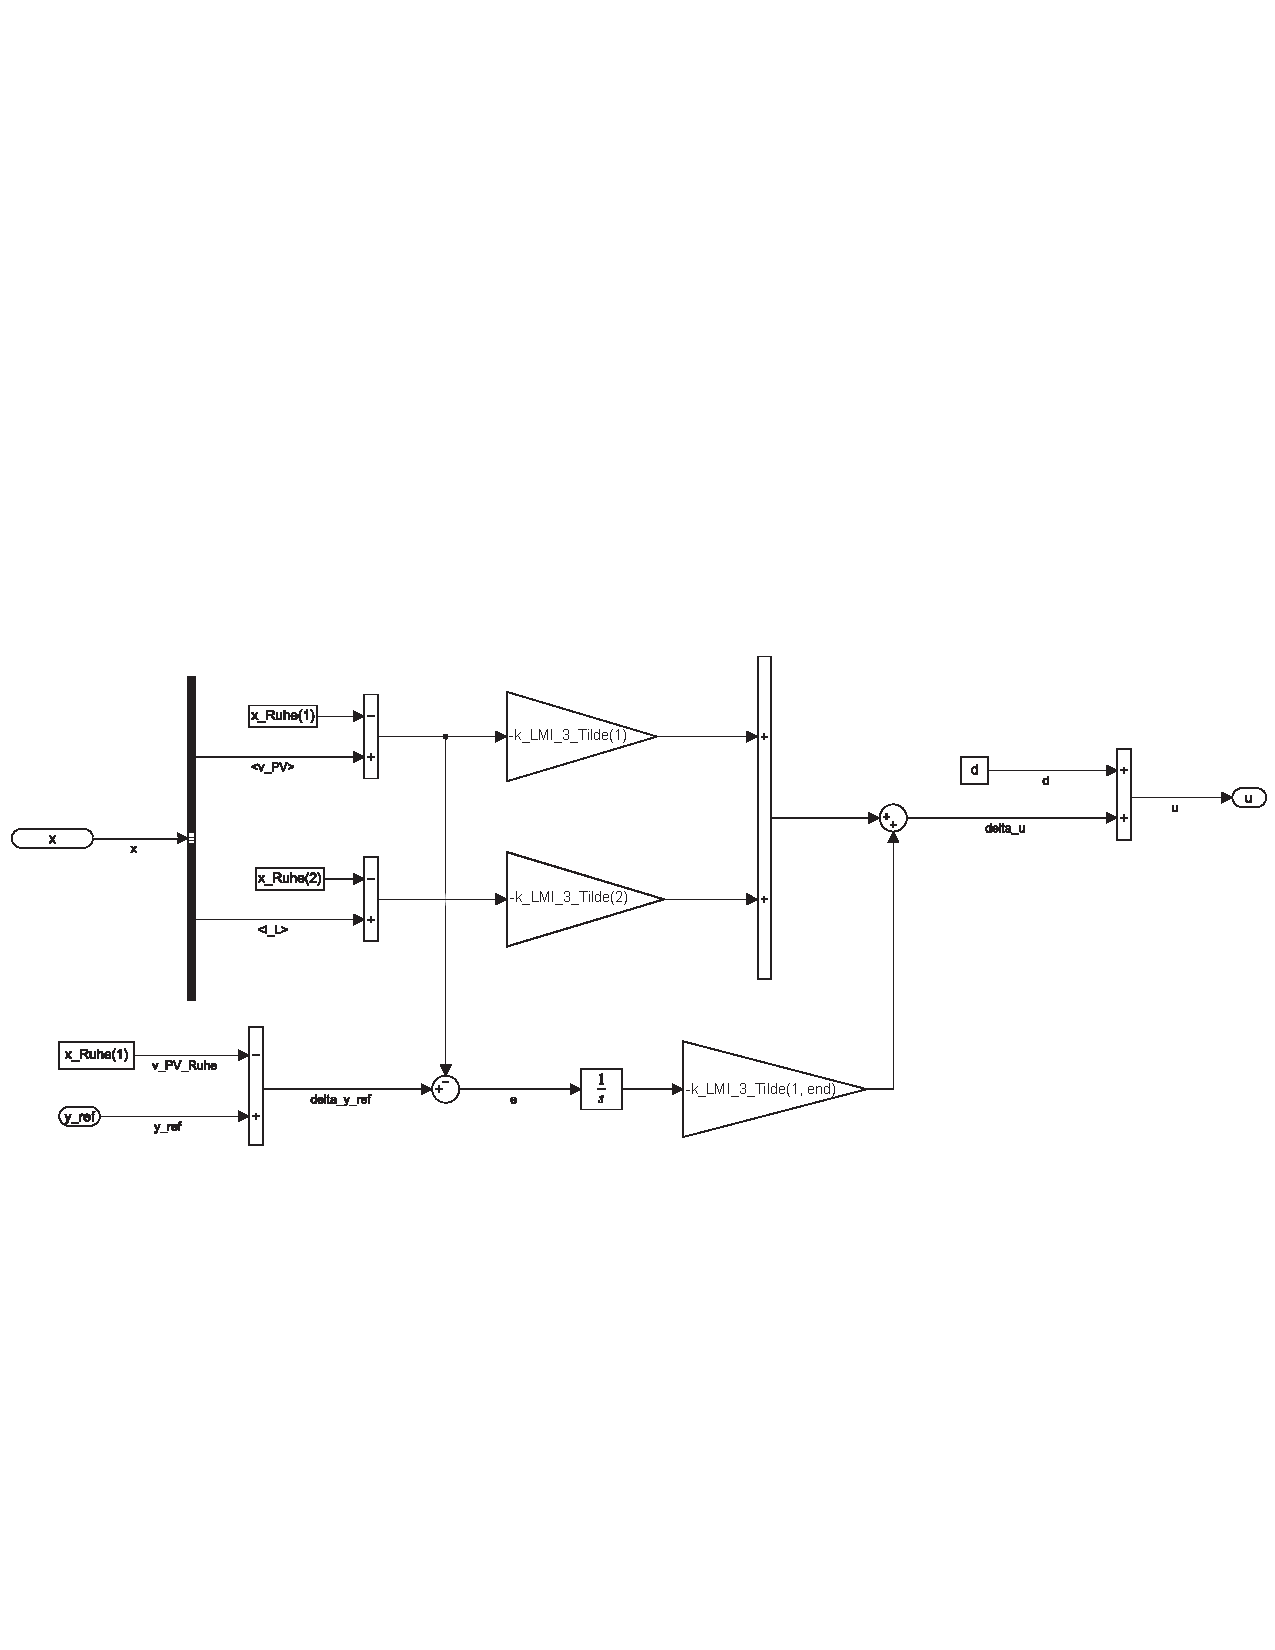
\includegraphics[width=1.0\textwidth]{Bilder/6_reglervalidierung/nichtlinear_i_regler_simu.pdf}}
    \caption[Zustandsregler mit I-Regelung Simulink (nichtlinear)]{Simulink Regler-Blockschaltbild für den Zustandsregler mit I-Regelung (nichtlineares Zustandsraummodell)}
    \label{fig:Bild24}
\end{figure}

Zur Validierung der Funktionsfähigkeit des Reglers wird erneut ein Referenzwert von $\SI{+10}{V}$ bezogen für die PV-Spannung $v_{\mathrm{PV,MPP}}$ vorgegeben. \autoref{fig:Bild25} zeigt nahezu identische Ergebnisse im Vergleich zum linearen Zustandsraummodell. Aufgrund dieser Erkenntnis wird auf weitere Analysen verzichtet.

\begin{figure}[H]
    \centering
    \fbox{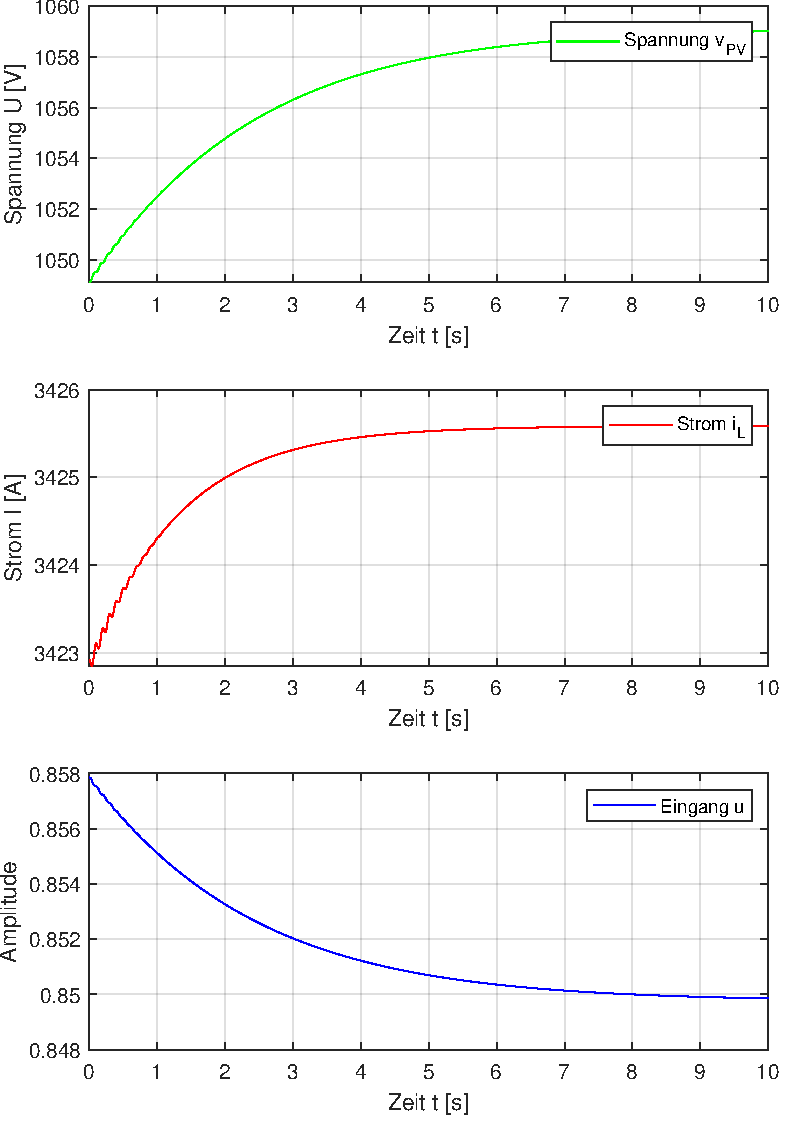
\includegraphics[width=0.85\textwidth]{Bilder/6_reglervalidierung/nichtlinear_i_regelung.pdf}}
    \caption[Validierung Regler mit I-Regelung (nichtlinear)]{$v_{\mathrm{PV}}$, $i_{\mathrm{L}}$ und $u$ bei $\alpha = 0.1$ und einem Referenzwert von $y_{ref} = v_{\mathrm{PV,MPP}} + \SI{10}{V}$ am Zustandsregler mit I-Regelung für das nichtlineare Zustandsraummodell}
    \label{fig:Bild25}
\end{figure}

\subsubsection{Vergleich des Regelverhaltens}

Abschließend kann festgehalten werden, dass die drei entwickelten Regler auch auf das nichtlineare Zustandsraummodell angewendet werden können und grundsätzlich plausible Ergebnisse produzieren. Bei der Referenzwertvorgabe für den Regler mit Vorsteuerung \bzw Regler mit I-Regelung konnte quantitativ ermittelt werden, dass die Performance der Zustandsregler nur für Referenzwerte von $y_{\mathrm{ref}} \in \mathbb{R} \: | \: \SI{-9}{V} \leq y_{\mathrm{ref}} \leq \SI{+12}{V}$ ausreicht. \\
Bis auf die Regelung mit Referenzwertvorsteuerung konnten annähern identische Kurvenverläufe im Vergleich zu den Simulationen am linearen Modell festgestellt werden. Besagte Unterschiede wurden bereits in \autoref{sec:val_nlin_vor} analysiert und festgehalten. Somit wird auf weitere Vergleiche an dieser Stelle verzichtet.

\begin{figure}[H]
    \centering
    \fbox{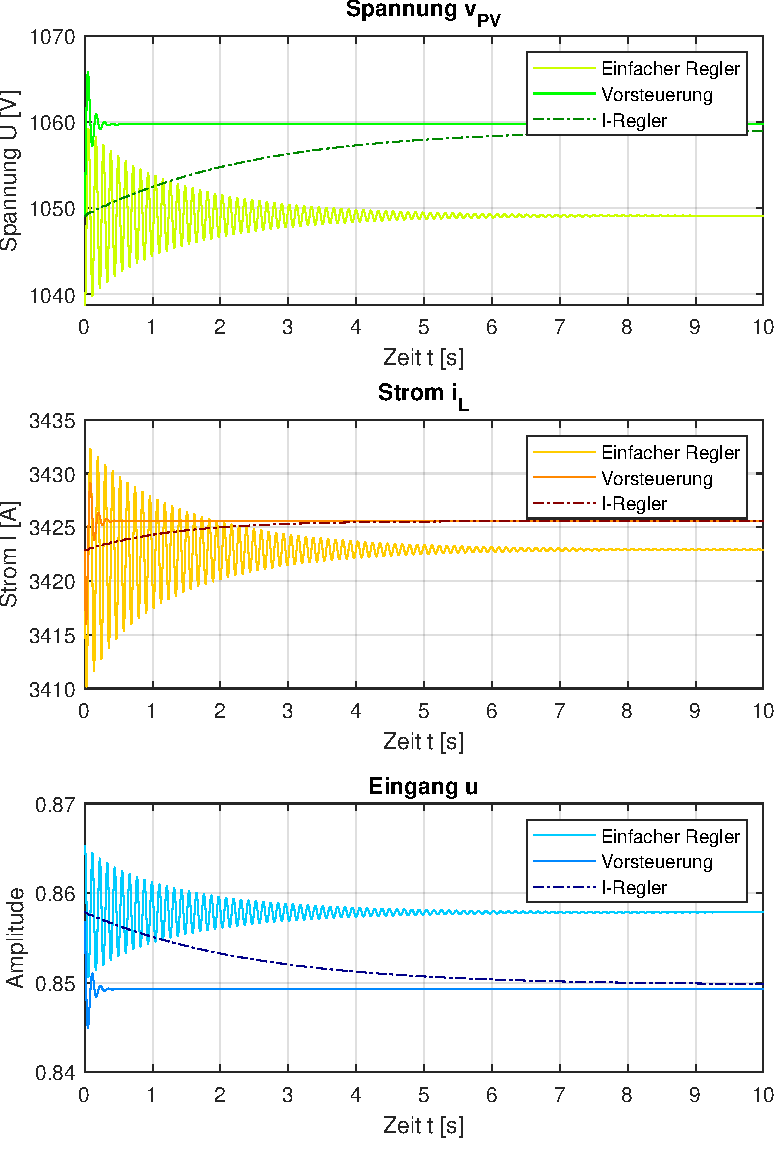
\includegraphics[width=0.8\textwidth]{Bilder/6_reglervalidierung/nichtlinear_reglervergleich.pdf}}
    \caption[Reglervergleich für das nichtlineare Zustandsraummodell]{$v_{\mathrm{PV}}$, $i_{\mathrm{L}}$ und $u$ für Regler mit einfacher Zustandsrückführung, Regler mit Referenzwertvorsteuerung und Regler mit I-Regelung bei einem Einganssprung von $v_{\mathrm{PV,MPP}} - \SI{10}{V}$ \bzw einem Referenzwert von $y_{ref} = v_{\mathrm{PV,MPP}} + \SI{10}{V}$ am nichtlinearen Zustandsraummodell}
    \label{fig:Bild26}
\end{figure}